%!!! cambiar esto por el diagrama de visio cuando este :)
\pagebreak
\section{Cursograma de Compras}
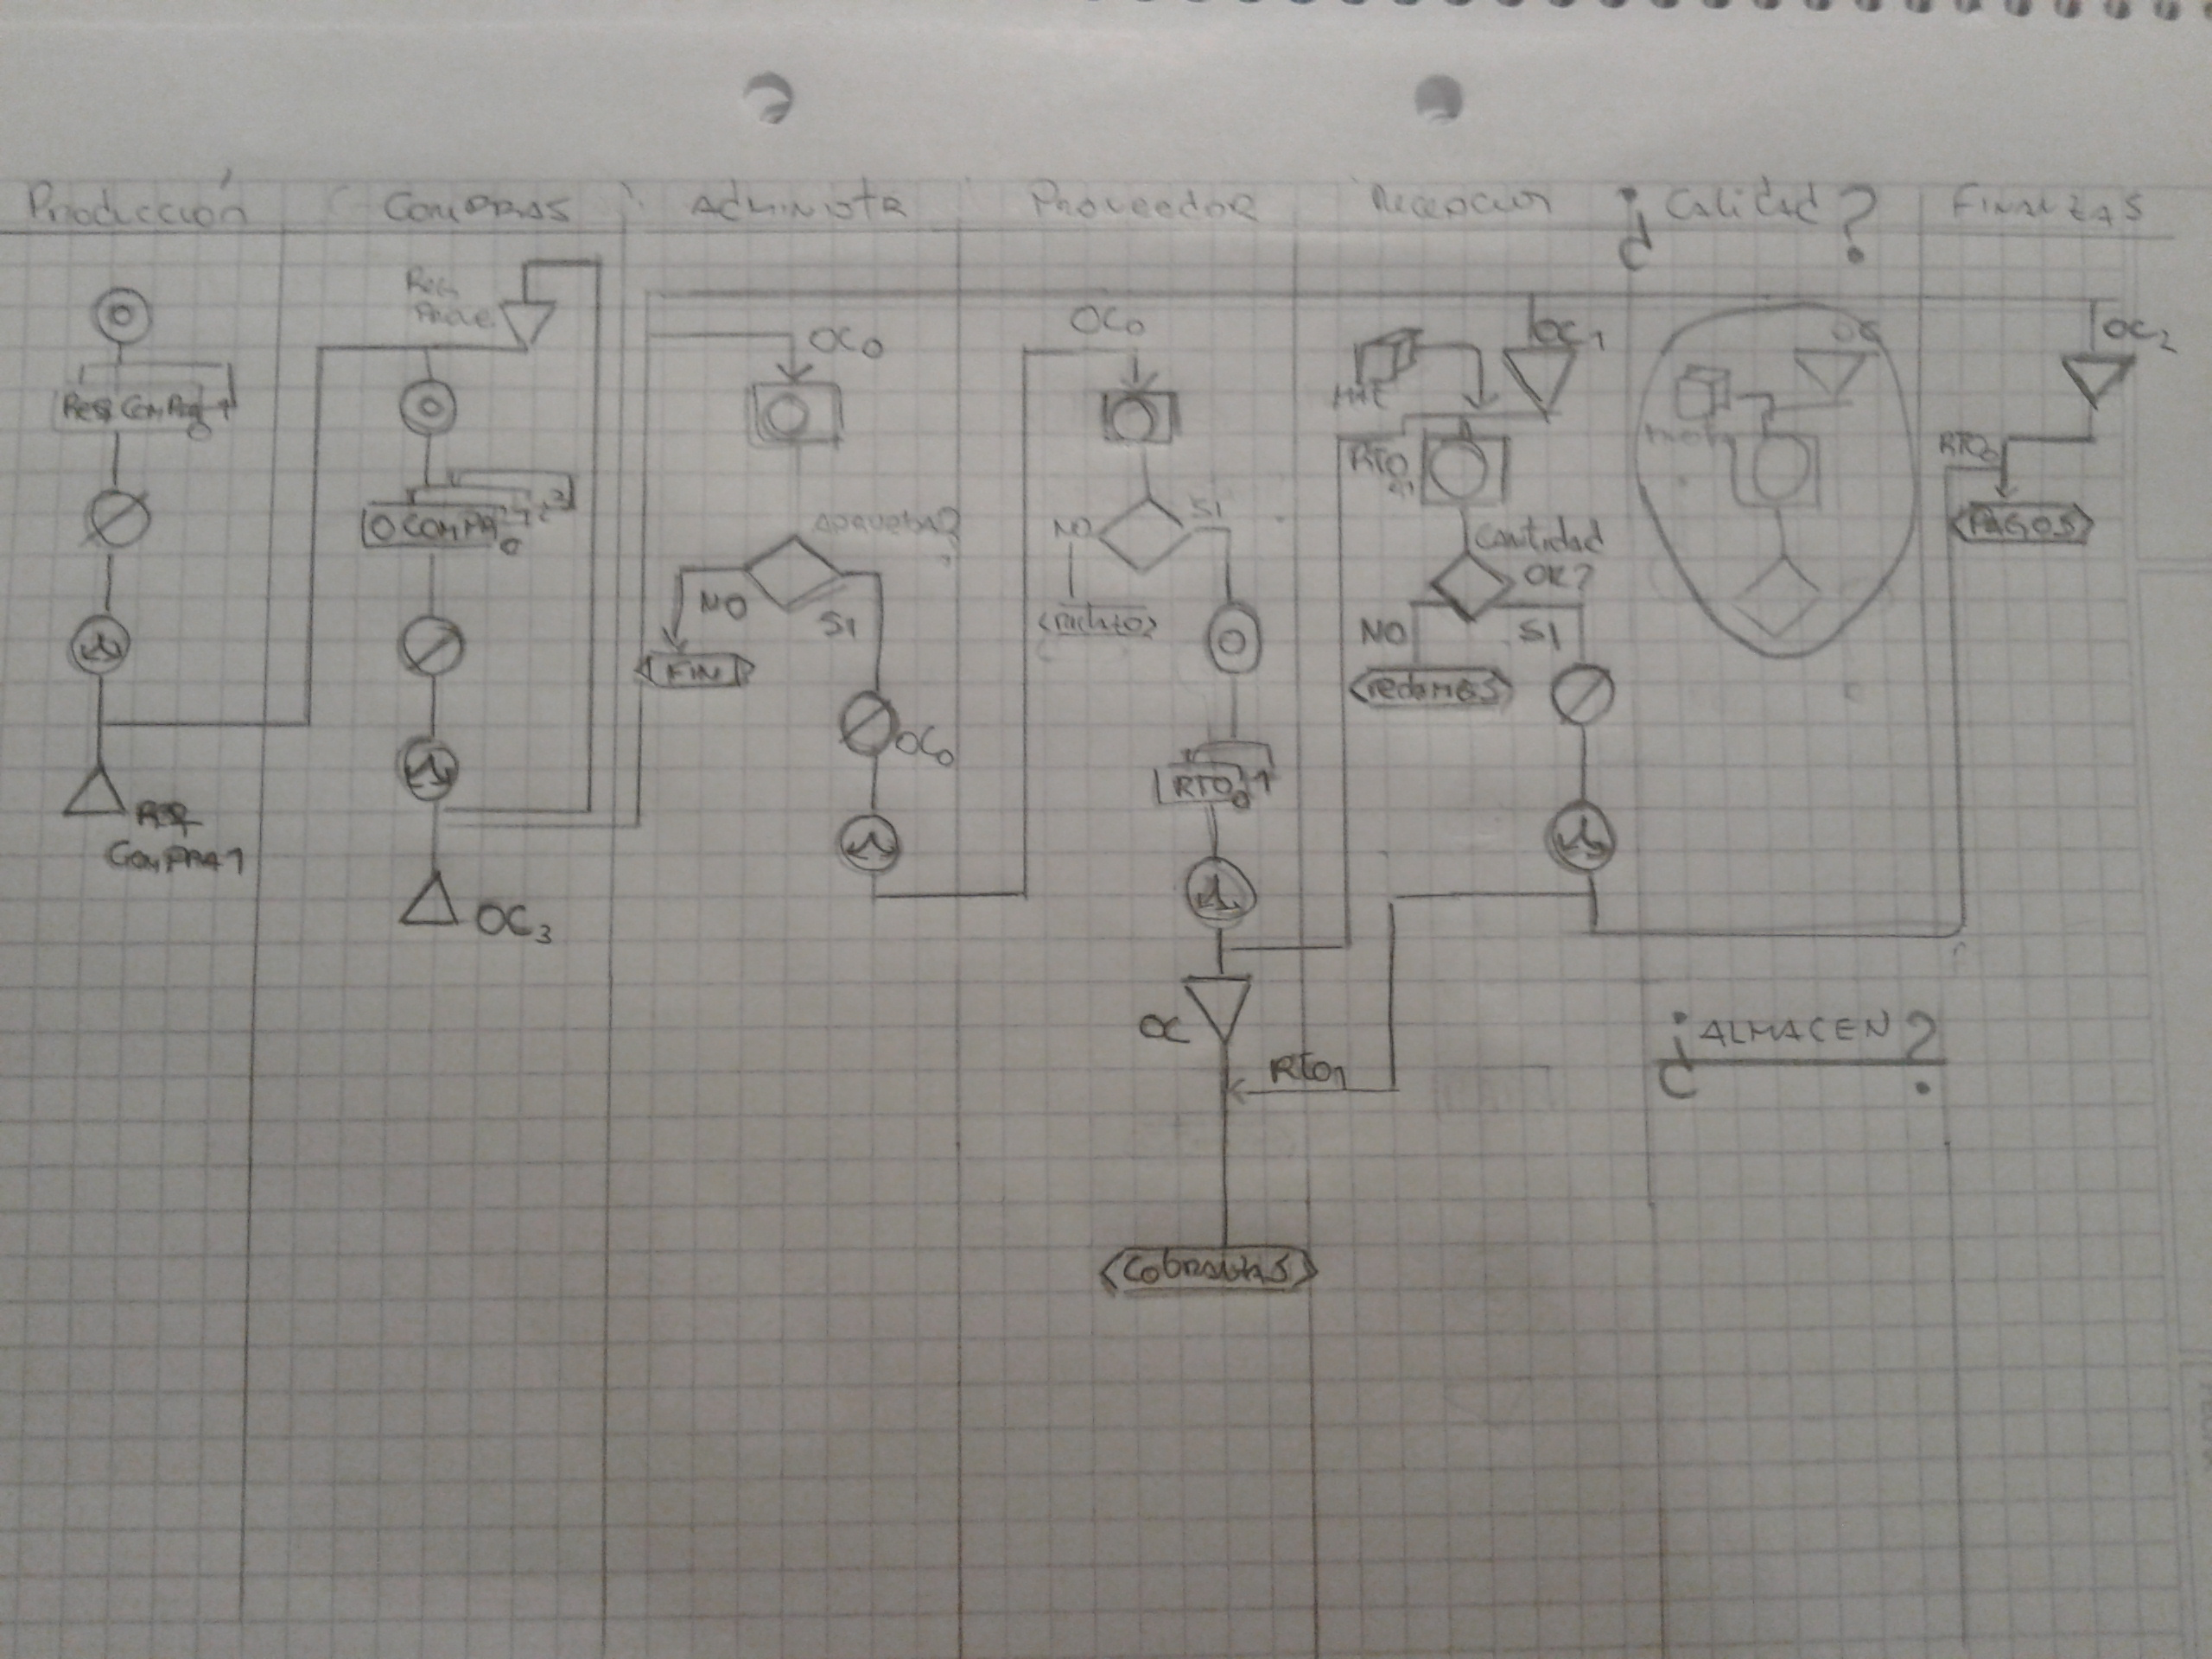
\includegraphics [scale=0.22 ,angle=90]{Empresa/Circuitos/Compras/Compras.jpg}

\pagebreak
\section{Procedimiento de Compras}
\begin{description}
\item[Producción] Tras detectar necesidad de materiales el sector de Producción emite un Pedido de Materiales (PM) en original y copia, el nivel autorizante firma el original y lo envía al sector de Almacenes, se archiva la copia.
\item[Almacenes] Tras recibir Pedido de Materiales del sector de Producción, Almacenes chequea las existencias y si tiene materiales suficientes los despacha; si no tiene los materiales necesarios, o se alcanza el punto de pedido, Almacenes emite un Requerimiento de Compra (RC) en original y copia, lo firma y envía al sector de Compras el original archivando la compra.
\item[Compras] Recibido el Requerimiento de Compra, el área de Compras consulta listas de precios del Registro de Proveedores, confeccionadas con Pedidos de Cotización realizados mensualmente, y en función de ellos confecciona una Orden de Compra (OC) original y tres copias, las firma y distribuye original a Dirección General, una copia a Recepción, una a Finanzas, una a Calidad y almacena la última copia.
\item [Dirección General] Tras recibir la Orden de Compra del sector de Compras, la Dirección General controla los precios contra Ordenes de Compra archivadas de compras anteriores, y en caso de aprobarla la firma y envía al sector de Ventas del Proveedor previamente seleccionado. En caso de rechazarla devuelve la Orden de Compra al sector de Compras para su revisión.
\item [Proveedor] Una vez recibida la Orden de Compra firmada por Compras y Dirección General el, Proveedor, según su circuito de ventas,  decide aceptar o rechazar la Orden de Compra. En caso de aceptarla, el Proveedor confecciona Remito (Rto) por duplicado y envía original y una copia junto con los materiales al sector de Recepción.
\item[Recepción] Tras recibir los materiales y el Remito original y una copia, el sector de Recepción controla cotejando cantidades en ambos contra la Orden de Compra. En caso de concordar, firma Remito original y copia, almacena temporalmente el original y devuelve la copia al Proveedor. Emite Pedido de Control (PC) en original y copia, envía la mercadería al sector de Calidad para su control junto con ambas copias del documento.
\item [Proveedor] Recibido el remito firmado continua con su Circuito no relevado de Cobranzas.
\item [Calidad] Recibida la mercadería de Recepción firma la copia del Pedido de Control y lo devuelve a Recepción. Controla la calidad contra lo especificado en el Pedido de Control y registra en el mismo el resultado del control. De aprobar, envía la mercadería a Almacenes. De no aprobar, devuelve la mercadería a Recepción para su devolución al Proveedor. En ambos casos firma el Pedido de Control y la envía a Recepción.
\item [Recepción] Tras recibir el Pedido de Control original, si está rechazado emite un Reclamo en original y copia, envía el original al Proveedor junto con la mercadería y archiva el Pedido de Control y el Remito originales. Si está aprobada, envía el Remito original a Finanzas. En ambos devuelve la copia del Pedido de Control a Calidad, quien la destruye.
\item [Finanzas] Una vez recibido el Remito original del sector de Recepción, procede a realizar el pago en el circuito no relevado de Pago a Proveedores.

\end{description}

\pagebreak
\section{Manual del Cursograma de Compras}

\pagebreak
\section{Formularios de Compras}
\subsection{Orden de Compra}
\begin{center}
 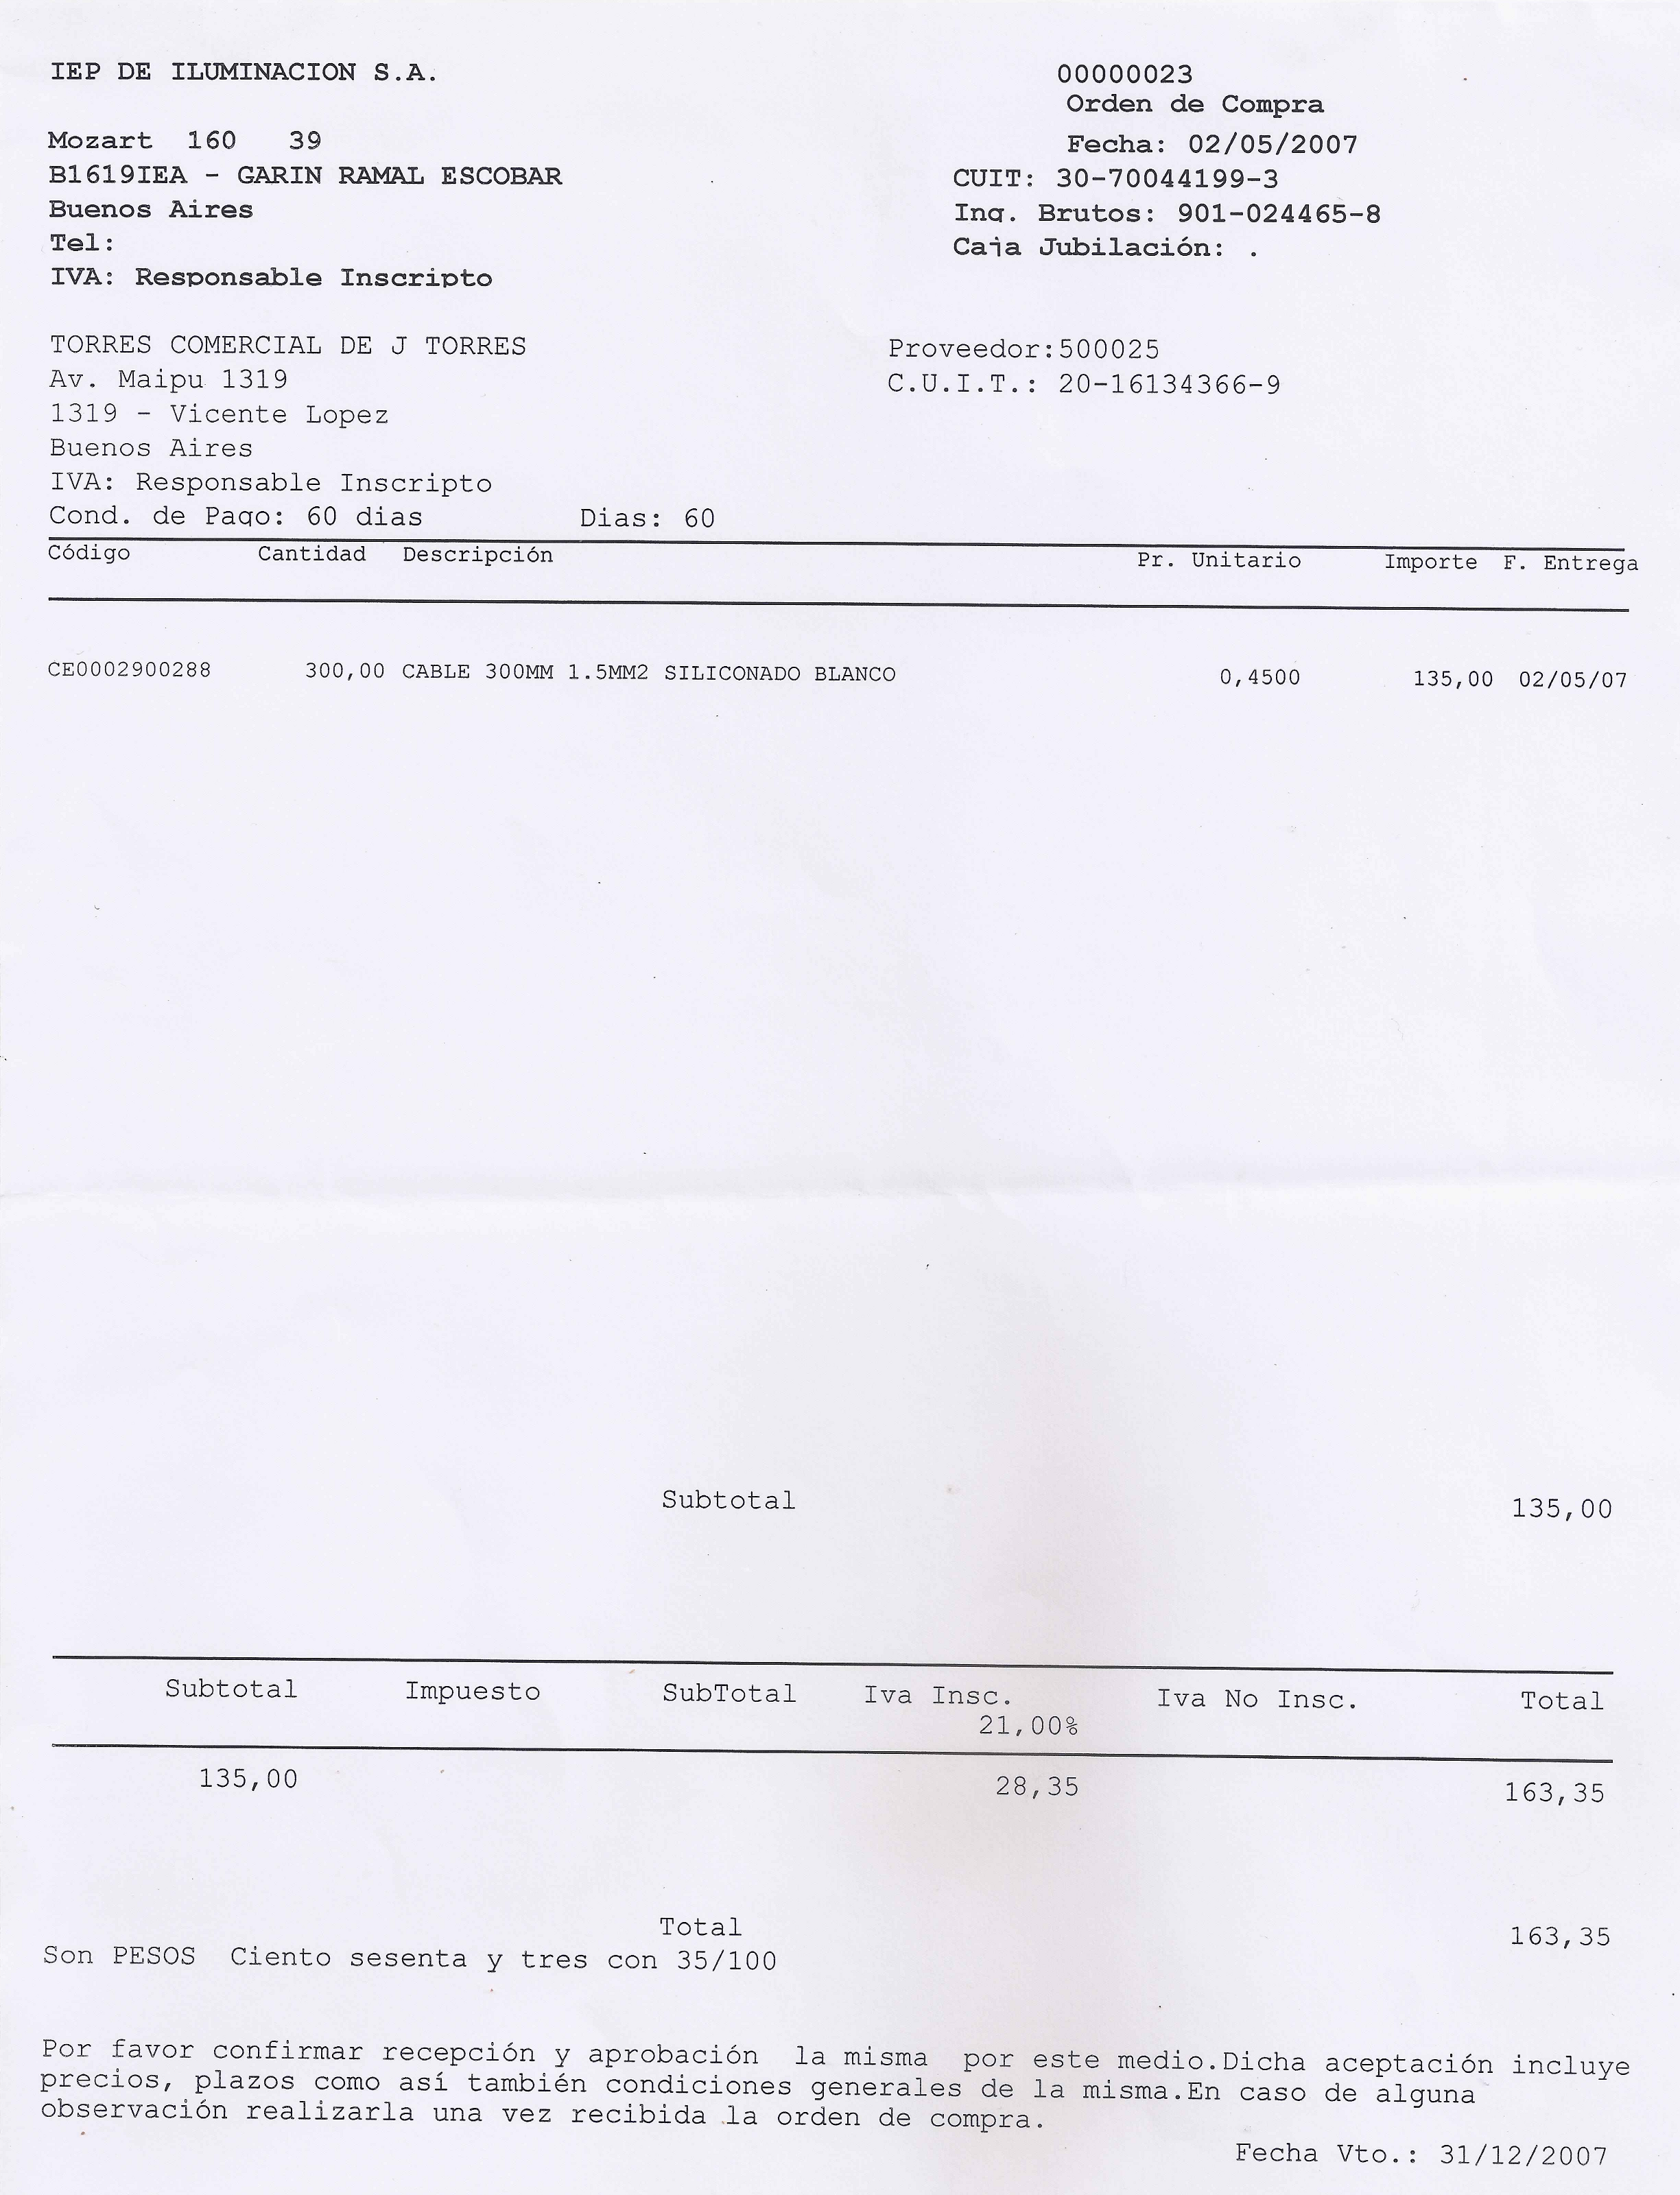
\includegraphics[scale=1.6,keepaspectratio=true]{./Images/FormulariosIEP/Orden-de-Compra.png}
 % Orden-de-Compra.png: 750x1002 pixel, 96dpi
\end{center}
\begin{itemize}
  \item \textbf{Objetivo:} Mediante este documento se comunica al proveedor la decisión de realizar una compra de materiales. Se especifican los productos a comprar con detalle de precios, cantidades, impuestos y condiciones de pago acordes a la previa cotización del proveedor.
  \item \textbf{Alcance:} Es un documento entre la empresa y su proveedor.
  \item \textbf{Emisor:} Compras
  \item \textbf{Cantidad de Copias Emitidas:} Original y 4 copias
  \item \textbf{Sector receptor:} Dirección General para su autorización y envío al proveedor
 \end{itemize}
\subsubsection{Descripci\'on campos de la Orden de Compra}
\begin{enumerate}
  \item Empresa emisora: Raz\'on Social de la empresa
  \item Empresa emisora: Informaci\'on de Sucursal. Domicilio y N\'umero de Tel\'efono
  \item Empresa emisora: Responsabilidad frente al IVA
  \item Número de Orden de Compra
  \item Fecha de emisi\'on
  \item Empresa emisora: CUIT y C\'odigo de Ingresos Brutos
  \item Proveedor: Raz\'on Social 
  \item Proveedor: Domicilio
  \item Proveedor: Responsabilidad frente al IVA
  \item Condici\'on de pago
  \item C\'odigo del proveedor al que se le compra
  \item Proveedor: CUIT
  \item Detalle de la Orden de Compra: C\'odigo del proveedor del \'item, Cantidad solicitada
  \item Detalle de la Orden de Compra: Descripci\'on del \'item
  \item Detalle de la Orden de Compra: Precio unitario del \'item
  \item Detalle de la Orden de Compra: Importe total del \'item (cantidad * precio unitario)
  \item Detalle de la Orden de Compra: Fecha de entrega del \'item
  \item Detalle de la Orden de Compra: Subtotal de items (suma de los totales de \'item)
  \item Resumen de la Orden de Compra: Subtotal de items (suma de los totales de \'item)
  \item Resumen de la Orden de Compra: Importe de impuestos que aplican (opcional)
  \item Resumen de la Orden de Compra: Subtotal después de impuestos (sólo si aplica impuestos)
  \item Resumen de la Orden de Compra: Gravamen de IVA para Inscriptos
  \item Resumen de la Orden de Compra: Gravamen de IVA para No Inscriptos
  \item Resumen de la Orden de Compra: Total después de IVA
  \item Importe Total de la Orden de Compra
  \item Importe Total de la Orden de Compra en letras
  \item Fecha de Vencimiento de la Orden de Compra
  \item Términos de confirmación de aprobación o rechazo
\end{enumerate}

\subsection{Formulario2}
imagen
\begin{itemize}
  \item \textbf{Objetivo:}
  \item \textbf{Alcance:}
  \item \textbf{Emisor:}
  \item \textbf{Cantidad de Copias Emitidas:}
  \item \textbf{Sector receptor:}
 \end{itemize}
\subsubsection{Descripci\'on campos del Formulario2}

\pagebreak
\section{Normas de Control Interno de Compras}
